%
% $Id: AttributeSet.java 15 2010-10-11 16:16:32Z justinkamerman $ 
%
% $LastChangedDate: 2010-10-11 13:16:32 -0300 (Mon, 11 Oct 2010) $ 
% 
% $LastChangedBy: justinkamerman $
%

\documentclass[10pt]{report}
\usepackage{graphicx}
\usepackage{setspace}			
\onehalfspacing

\title{CS6999 Programming Assignment 1}
\author{Justin Kamerman 3335272}
\date{\today}

\begin{document}
\maketitle
% No chapter numbers
\renewcommand*\thesection{\arabic{section}}

%----------------------------------------
% Assignment
%----------------------------------------
\section*{Assignment}
\begin{enumerate} 
\item Implement the Aho-Corasick string matching algorithm\cite{RefWorks:103} and test its performance for:
  \begin{itemize}
  \item 1000 blogs and  100 keywords
  \item 2,000 blogs and 100 keywords
  \item 4,000 blogs and 100 keywords
  \item 8,000 blogs and 100 keywords
  \item 16,000 blogs and 100 keywords
  \item 32,000 blogs and 100 keywords
  \end{itemize}
           
Repeat the experiments for 200 and 400 keywords.
      

\item Build an inverted index for 10, 000 blogs. Use 10 keywords to query the index to:
  \begin{itemize}
  \item Locate each keyword and retrieve their corresponding blogs.
  \item Show the intersection of every two keywords. For example, retrieve the document ID of the blogs that keywords 1 and 2 have occurred together at least once. Similarly, for keywords 1 and 3, ..., keywords 2 and 3, keywords 2 and 4, ...
    \item Similarly, show the intersection of every 3 keywords, 4 keywords, etc.
  \end{itemize}
  
\item Do a comparative analysis (time to build the index and time to retrieve) of the two methods.
\end{enumerate}

%----------------------------------------
% Aho-Corasick Algorithm
%----------------------------------------
\section{Aho-Corasick Algorithm}
\label{sec:ahocorasickalgorithm}
The Aho-Corasick string matching algorithm\cite{RefWorks:103} is a
kind of dictionary matching search algorithm that constructs a finite
state machine to scan for a given set of keywords. It is, in effect, a
reduced grammar regular expression parser described in
\cite{RefWorks:111}. In our search implementation, the finite state
machine is constructed given a list of keywords and then the documents
of the test corpus are read from secondary storage and fed through the
finite state machine. As soon as a document is found to contain at
least one instance of a set of search terms, parsing of that document
ends.

The documents of the corpus are each stored in a disk file, named for
the identifier of the original blog extract. In an attempt to exploit
the fact that reading documents from disk is slower than state machine
scanning, the scan process uses a thread pool to read and parse
multiple documents concurrently. By expanding the thread pool, the
implementation is able to achieve higher CPU utilization and marginal
improvements in search times. However, the limits of the experiment
platform did not accommodate increasing the pool size to a point where
the added synchronization issues were justified.


\subsection*{Implementation}
The Aho-Corasick algorithm are implemented by a Java
program. The only external dependency is on the Apache commons-cli
library for parsing commend line options. To that end, the program is
operated from the command line, taking options listed in table
~\ref{tab:ahocommandline}.  
\\
\begin{table}[h]
  \centering
  \begin{tabular}{ |l|p{10cm}|} 
    \hline
    Option & Description \\ \hline
    -d \<arg\>  &  Document directory \\ \hline
    -k \<arg\>  &  Keywords file \\ \hline
    -p \<arg\>  &  Thread pool size. Default is 10 \\ \hline
    -g          &  Generate DOT visulaization of state machine \\ \hline
    -h          &  Print help message \\ \hline
  \end{tabular}
  \caption{Command line options for Aho-Corasick implementation}
  \label{tab:ahocommandline}
\end{table}
\\

The program implements various mechanism to facilitate
debugging. Throughout the code, log statements have been added using
the Java logging framework. The logging output is controlled for
individual classes via the \texttt{logging.properties} file which the
program read on startup. In addition to logging, code was added to
generate Graphviz DOT\cite{RefWorks:110} output
representing the state machine created. A sample \textit{dot} file for the state machine generated for the four
keywords used in \cite{RefWorks:103} (\textit{he, she, his, hers}), is
shown below. The associated image generated by DOT is shown in figure
\ref{fig:dot}.


\begin{verbatim}
digraph G {
	0  [label="0 []", shape=circle];
	0 -> 3 [label="s"];
	0 -> 1 [label="h"];
	1  [label="1 []", shape=circle];
	1 -> 2 [label="e"];
	1 -> 6 [label="i"];
	1 -> 0 [color="red"];
	6  [label="6 []", shape=circle];
	6 -> 7 [label="s"];
	6 -> 0 [color="red"];
	7  [label="7 [his]", shape=circle];
	7 -> 3 [color="red"];
	2  [label="2 [he]", shape=circle];
	2 -> 8 [label="r"];
	2 -> 0 [color="red"];
	8  [label="8 []", shape=circle];
	8 -> 9 [label="s"];
	8 -> 0 [color="red"];
	9  [label="9 [hers]", shape=circle];
	9 -> 3 [color="red"];
	3  [label="3 []", shape=circle];
	3 -> 4 [label="h"];
	3 -> 0 [color="red"];
	4  [label="4 []", shape=circle];
	4 -> 5 [label="e"];
	4 -> 1 [color="red"];
	5  [label="5 [she, he]", shape=circle];
	5 -> 2 [color="red"];
}
\end{verbatim}

\begin{figure}
  \begin{center}
	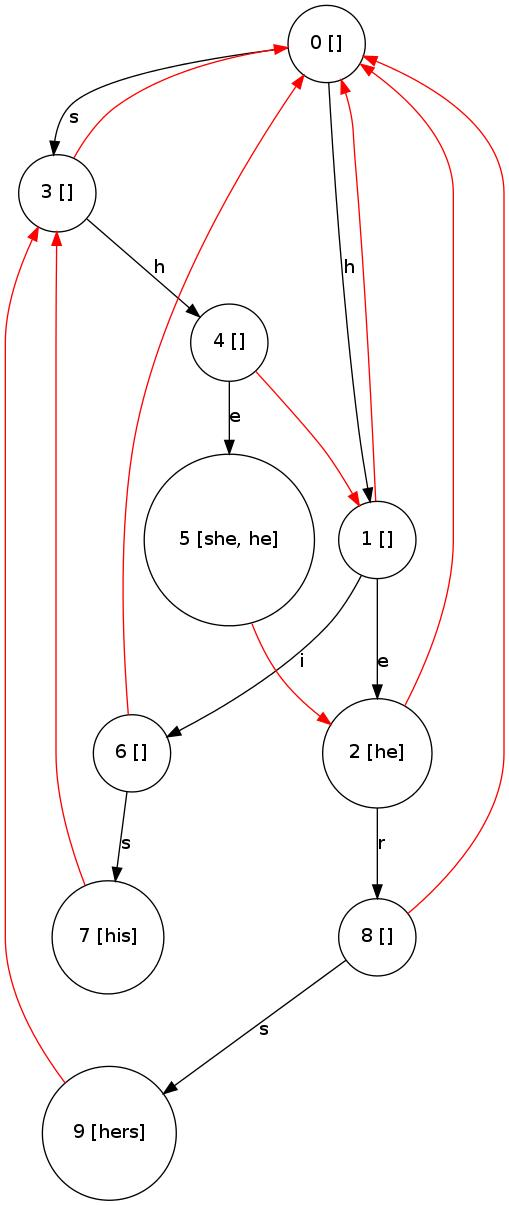
\includegraphics[width=!,height=0.90\textheight]{aho4}
  \end{center}
  \caption{Aho-Corasick state machine visualization generated by DOT}
  \label{fig:dot}
\end{figure} 

\begin{figure}
  \begin{center}
	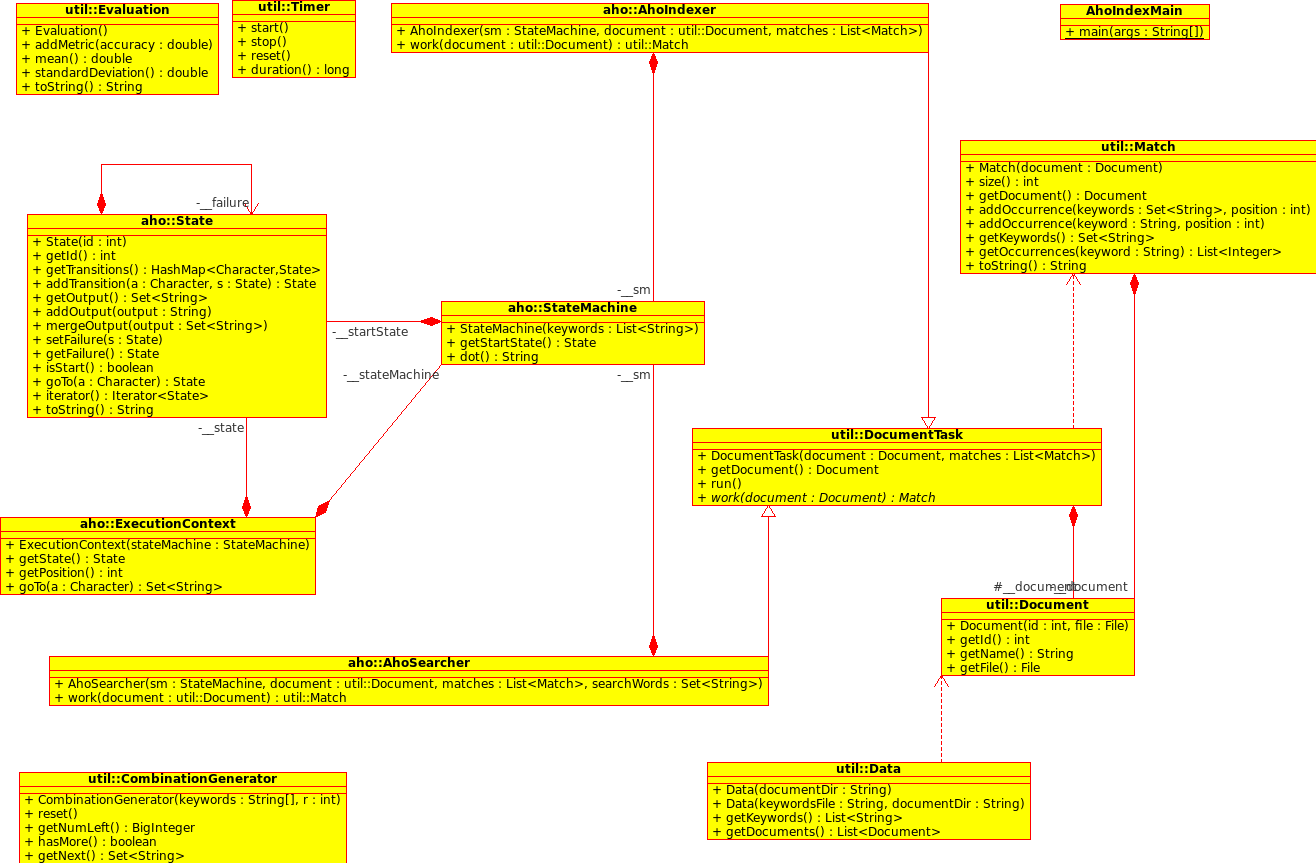
\includegraphics[angle=90,width=\textwidth,height=!]{ahouml}
  \end{center}
  \caption{Aho-Corasick Implementation UML class diagram}
  \label{fig:ahouml}
\end{figure} 

The implementation classes and their relationships are represented in a UML
class diagram in Figure \ref{fig:ahouml}. Following is a brief
description of each class:

\begin{itemize}
\item \textbf{AhoIndexMain}

\item \textbf{AhoSearchMain} 

\item \textbf{AhoIndexer}

\item \textbf{AhoSearcher} 

\item \textbf{CombinationGenerator}

\item \textbf{Evaluation}

\item \textbf{ExecutionContext} 

\item \textbf{StateIterator} 

\item \textbf{StateMachine} 

\item \textbf{Data} 

\item \textbf{Document} 

\item \textbf{DocumentTask} 

\item \textbf{LogFormatter} is a helper class to format log messages.

\item \textbf{Match}

\item \textbf{Timer}

\end{itemize}


\subsection*{Results}
Various tests were conducted to characterise the performance of the
Aho-Corasick search algorithm:

\begin{itemize}
\item The time taken to construct the Aho-Corasick state machnie was
  measured for different numbers of keywords. The results of this test
  is shown in figure \ref{fig:ahostatemachine}. TODO

\item The time taken for the Aho-Corasick state machine to scan
  different sized corpora was measured. The test was repeated for
  various state machines, contructed using a 100, 200, and 400 keyword
  set. The results of this test are shown on figure
  \ref{fig:ahoscan}. TODO

\item The time taken to search for different numbers of keywords was
  measured over different sized corpora. A set of ten
  keywords was selected randomly and the the corpora searched for ${n
    \choose k}$ enumerated combinations thereof to obtain an average
  for a particular keyword set size. The results of this test are
  shown in figure \ref{fig:ahosearch}. TODO
\end{itemize}


\begin{figure}
  \begin{center}
	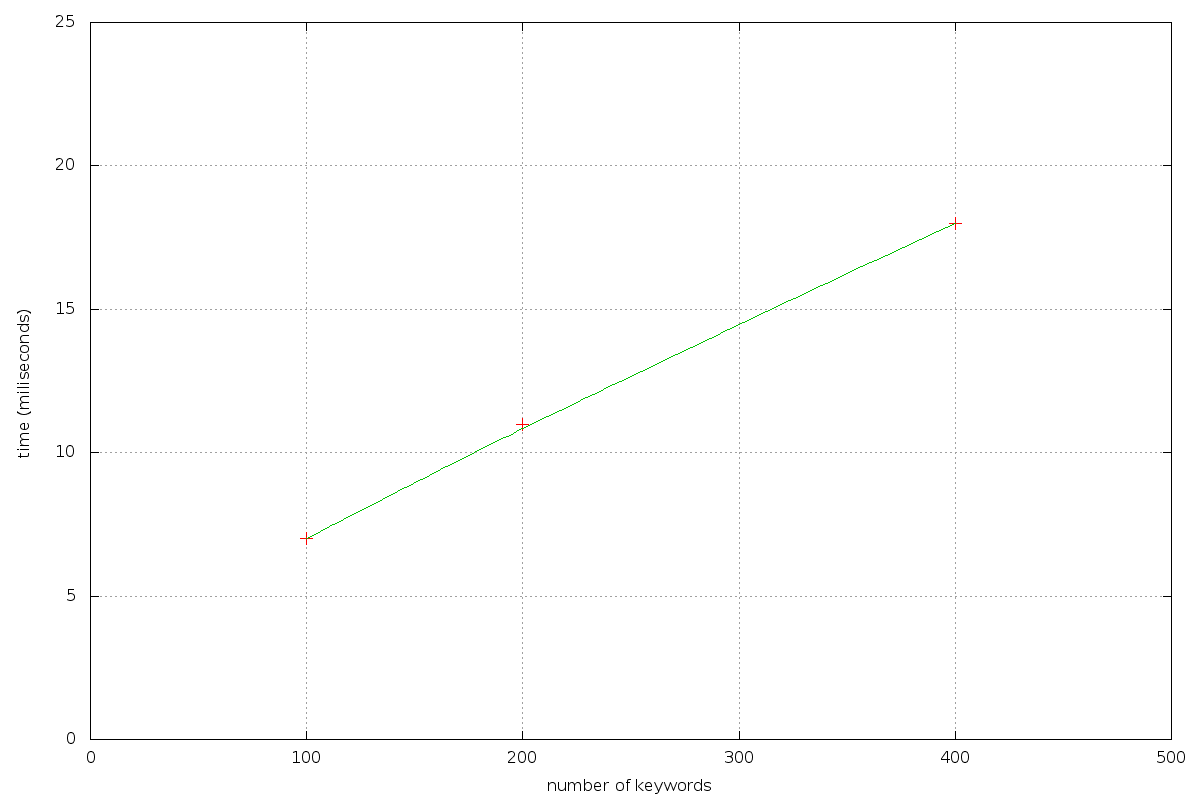
\includegraphics[width=\textwidth,height=!]{ahostatemachine}
  \end{center}
  \caption{Aho-Corasick state machine construction}
  \label{fig:ahostatemachine}
\end{figure} 

\begin{figure}
  \begin{center}
	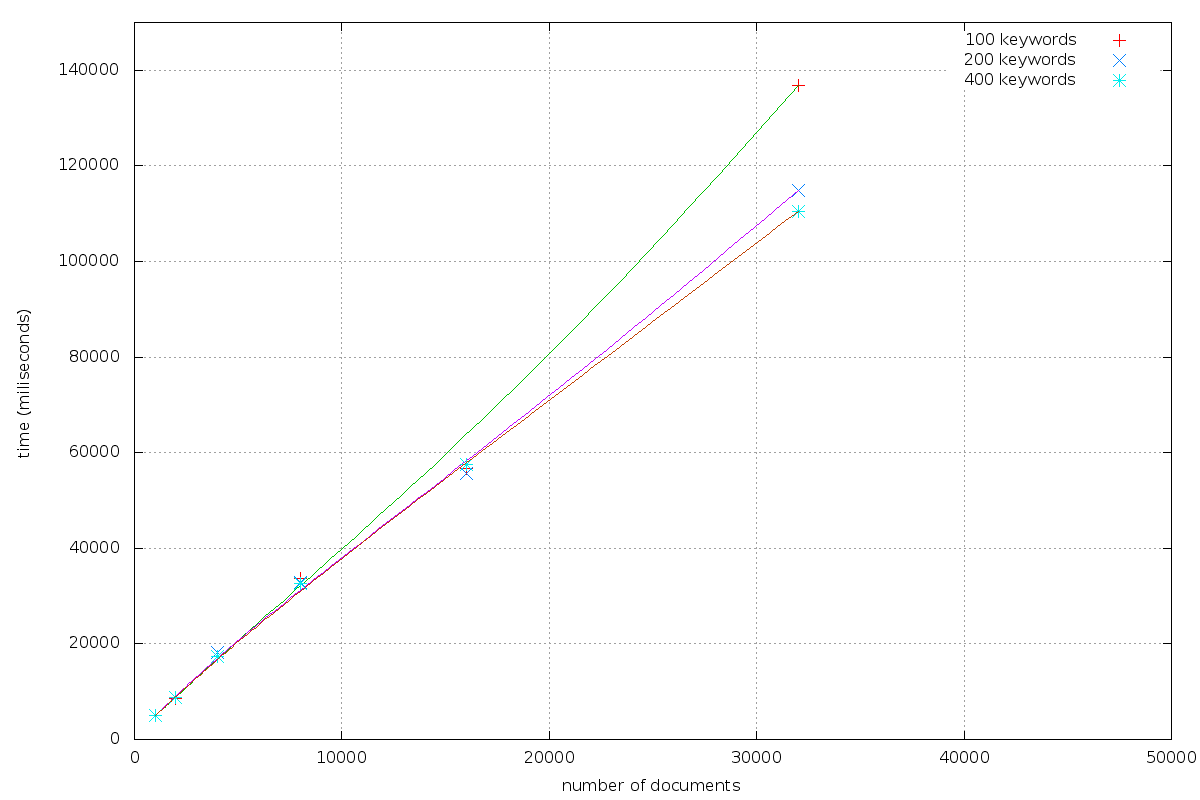
\includegraphics[width=\textwidth,height=!]{ahoscan}
  \end{center}
  \caption{Aho-Corasick state machine scanning}
  \label{fig:ahoscan}
\end{figure} 

\begin{figure}
  \begin{center}
	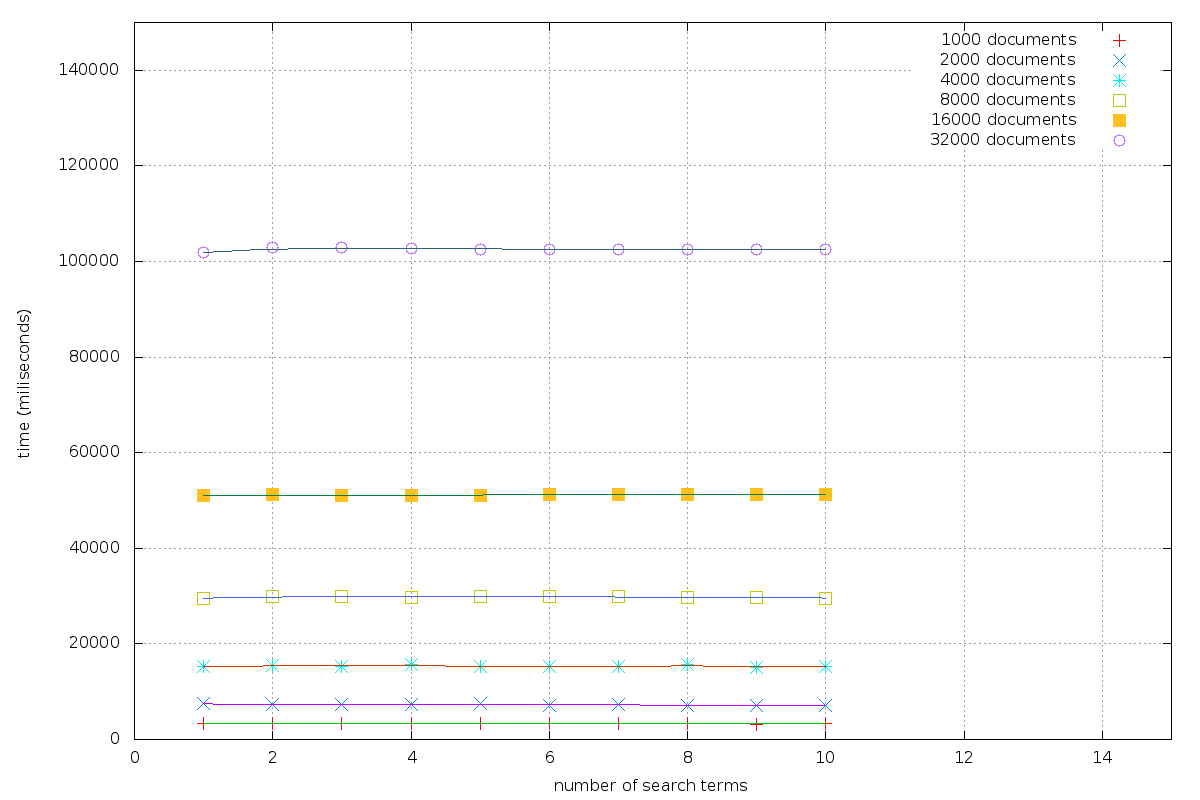
\includegraphics[width=\textwidth,height=!]{ahosearch}
  \end{center}
  \caption{Aho-Corasick state machine search}
  \label{fig:ahosearch}
\end{figure} 

%----------------------------------------
% Inverted Index
%----------------------------------------
\section{Inverted Index}
The program builds an \textit{inverted index} of a given corpus for
boolean search. The implementation is based on the techniques and
methods described in \cite{RefWorks:109}. A lexical scanner generator,
\textit{JLex}\cite{RefWorks:112}, is used to generate a scanner which
is used to construct a term index each document. The scanner is
configured to ignore a list of 430 stop words. The term indices for
each document are post-processed to construct an inverted index
mapping each term to a list of documents containing the term.

The documents of the corpus are each stored in a disk file, named for
the identifier of the original blog extract. In an attempt to exploit
the fact that reading documents from disk is slower than state machine
scanning, the index creation process uses a thread pool to read and
parse multiple documents concurrently. By expanding the thread pool,
the implementation is able to achieve higher CPU utilization and
marginal improvements in index construction times. However, the limits
of the experiment platform did not accommodate increasing the pool
size to a point where the added synchronization issues were justified.


\subsection*{Implementation}
The \textit{inverted index} is generated by a Java
program. The only external dependency is on the Apache commons-cli
library for parsing commend line options. To that end, the program is
operated from the command line, taking options listed in table
~\ref{tab:invcommandline}.  
\\
\begin{table}[h]
  \centering
  \begin{tabular}{ |l|p{10cm}|} 
    \hline
    Option & Description \\ \hline
    -d \<arg\>  &  Document directory \\ \hline
    -p \<arg\>  &  Thread pool size. Default is 10 \\ \hline
    -h          &  Print help message \\ \hline
  \end{tabular}
  \caption{Command line options for inverted index implementation}
  \label{tab:invcommandline}
\end{table}
\\

The program implements various mechanism to facilitate
debugging. Throughout the code, log statements have been added using
the Java logging framework. The logging output is controlled for
individual classes via the \texttt{logging.properties} file which the
program reads on startup.

\begin{figure}
  \begin{center}
	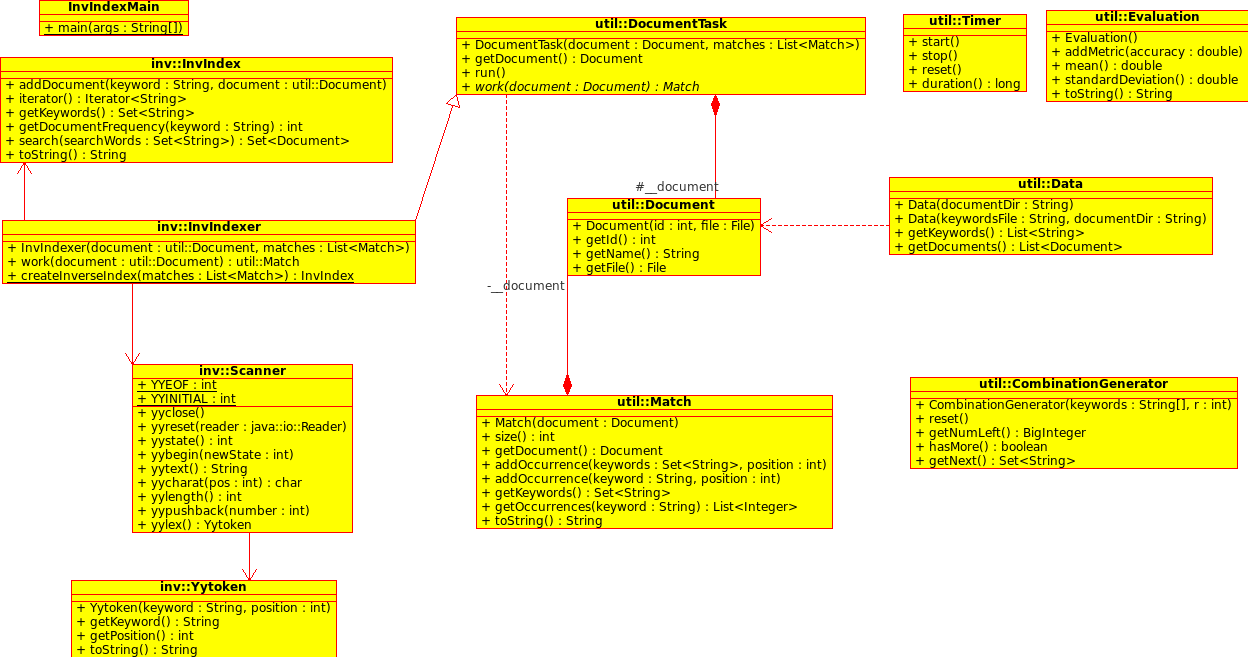
\includegraphics[angle=90,width=!,height=0.90\textheight]{invuml}
  \end{center}
  \caption{Inverted Index Implementation UML class diagram}
  \label{fig:invuml}
\end{figure} 

The implementation classes and their relationships are represented in a UML
class diagram in Figure \ref{fig:invuml}. Following is a brief
description of each class:

\begin{itemize}
\item \textbf{CombinationGenerator}

\item \textbf{Evaluation}

\item \textbf{ExecutionContext} 

\item \textbf{InvIndexMain}

\item \textbf{InvIndexer}

\item \textbf{AhoSearcher} 

\item \textbf{Data} 

\item \textbf{Document} 

\item \textbf{DocumentTask} 

\item \textbf{LogFormatter} is a helper class to format log messages.

\item \textbf{Match}

\item \textbf{Timer}

\end{itemize}


\subsection*{Results}
Various tests were conducted to characterise the performance of the inverted index search algorithm:

\begin{itemize}
\item The time taken to construct the inverted index was measured for different sized corpora. The results of this test is shown in figure \ref{fig:invscan}. TODO

\item The time taken to search for different numbers of keywords was measured over different sized corpora. A set of ten keywords was selected randomly and the the corpora searched for ${n \choose k}$ enumerated combinations thereof to obtain an average for a particular keyword set size. The results of this test are shown in figure \ref{fig:invsearch}. TODO
\end{itemize}


\begin{figure}
  \begin{center}
	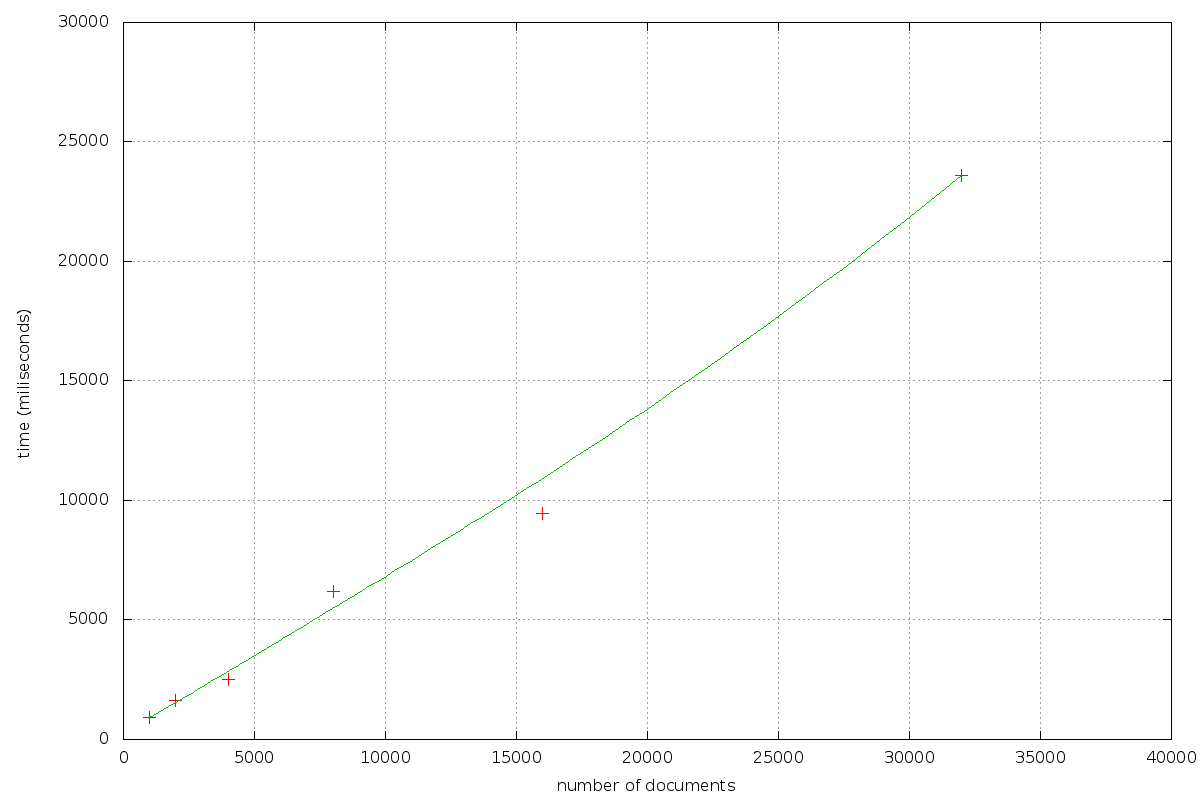
\includegraphics[width=\textwidth,height=!]{invscan}
  \end{center}
  \caption{Inverted index creation}
  \label{fig:invscan}
\end{figure} 

\begin{figure}
  \begin{center}
	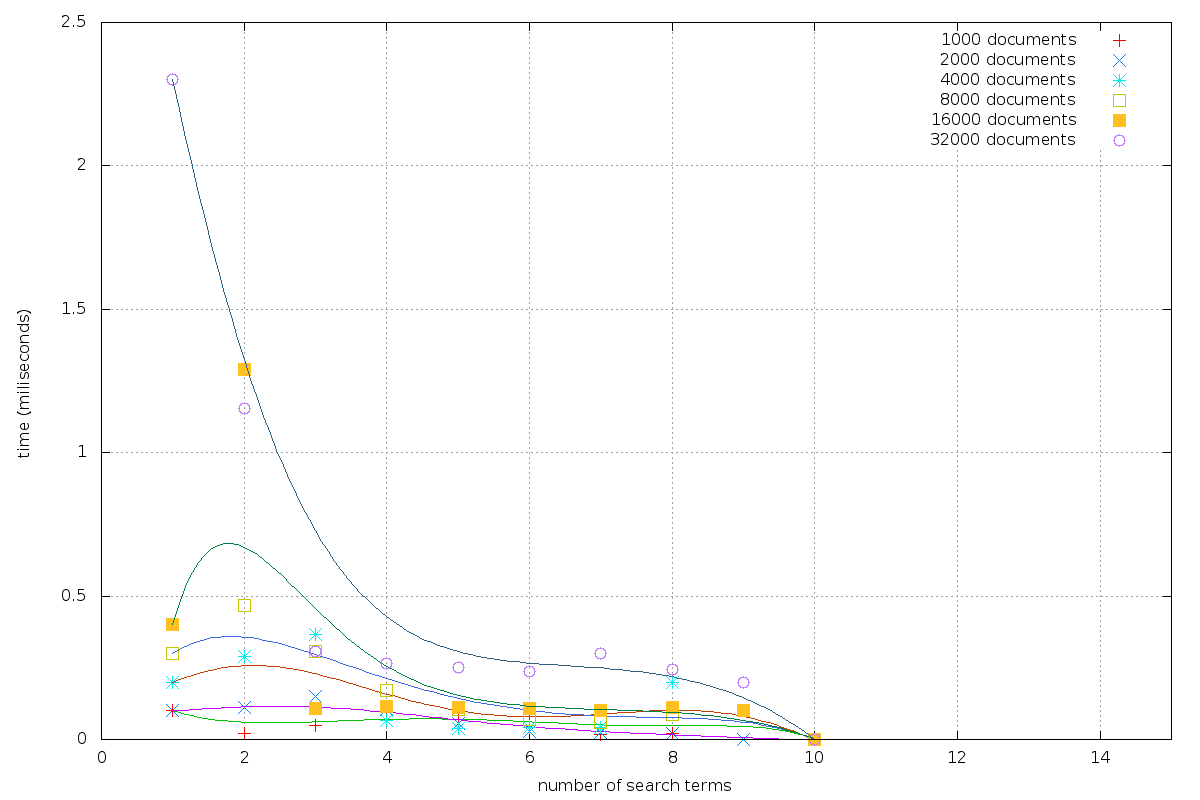
\includegraphics[width=\textwidth,height=!]{invsearch}
  \end{center}
  \caption{Inverted index search}
  \label{fig:invsearch}
\end{figure} 

%----------------------------------------
% Algorithm Comparison
%----------------------------------------
\subsection*{Algorithm Comparison}
\label{sec:algorithmcomparison}
All tests were run on a Dell laptop with an Intel Core Duo 2GHz
processor, 1GB RAM, running a 32 bit Linux 2.6.37 kernel. The Java
Virtual Machine used was version 1.6.0-24. 


%----------------------------------------
% Bibliography
%----------------------------------------
\bibliography{bibliography}
\bibliographystyle{IEEEannot}


%--------------------------------------------------
\end{document}
